%\documentclass{elsarticle}
%%
\documentclass[times,12pt,3p,longtitle]{elsarticle}
\usepackage{makecell}

%%
\usepackage{hyperref}
\hypersetup{
    colorlinks=true,
    linkcolor=blue,
    filecolor=magenta,      
    urlcolor=cyan,
    pdftitle={Overleaf Example},
    pdfpagemode=FullScreen,
    }

%% Stylefile to load JCOMP template
%% The amssymb package provides various useful mathematical symbols
\usepackage{amssymb}
\usepackage{latexsym}
%\journal{Journal of Computational Physics}
\usepackage{amsmath}
\begin{document}

\begin{frontmatter}
\title{A hybrid Eulerian-Lagrangian Vlasov method for nonlinear wave-particle interaction in weakly inhomogeneous magnetic field}
\author[1]{Jiangshan Zheng}

\author[2]{Ge Wang}
\author[1]{Bo Li}
\address[1]{School of Physics, Beihang University, Beijing, Beijing 100191, China}
\address[2]{Institute for Fusion Studies, The University of Texas, Austin, Texas, 78712, USA}
\begin{abstract}
  We present a hybrid Eulerian-Lagrangian Vlasov solver for nonlinear resonant wave-particle interactions problems in weakly inhomogeneous magnetic field.
  The governing Vlasov equation is derived from a recently proposed resonance tracking Hamiltonian method. 
  The method tracks the dynamics of deeply trapped resonant particles in a coherent wave. 
  It gives the evolution of the distribution function with a scale separated Hamiltonian that containing the slowly-varying motion about the resonant frame of reference and fast-varying coherent interactions.
  The hybrid method solves the slowly-varying phase space dynamics by Lagrangian method along the resonant trajectory, while simultaneously manages the fast-varying phase-space evolution in Eulerian grid with an adaptive time step interpolated differential operator scheme.
  We apply our method to study the frequency chirping problem of whistler mode chorus wave in the Earth magnetosphere and successfully reproduce the chirping chorus wave. 
  The results in well agree with previous research. 
  With a focus on nonlinear resonant wave-particle interaction in the weakly inhomogeneous regime, our approach can give high resolution for the fast varying phase space at low computational cost.  
  It could provide additional insights of the wave instabilities and particle energy transfer compared to the conventional Vlasov and particle-in-cell methods.
\end{abstract}
%xtend the periodical condition in the resonance frame
\end{frontmatter}
%\linenumbers

%main text
\clearpage

%intro the wave and the vlasov
\section{Introduction}
Wave-particle interaction, especially the nonlinear resonant interaction, is of great importance and has been extensively discussed in a broad spectrum of plasma physics. 
In magnetically confined fusion devices, the Alfv\'en wave instabilities 
are associated with mode frequency sweeping 
\cite{chen2016,wang2018,wang2012,wang2012a} 
and lead to premature ejection of alpha particles that deteriorate plasma confinement \cite{fasoli2007}.
The chorus waves  
in the planetary magnetosphere \cite{tsurutani1974} 
%as well as in the laboratory devices \cite{vancompernolle2015,vancompernolle2017a}
%, researchers have studied 
are associated with various geophysical activity like relativistic electron precipitation, X-ray microbursts, pulsating and diffuse auroras \cite{kasahara2018,reeves2013,thorne2013}.
%It has been demonstrated that the nonlinear resonant interaction between toroidal Alfv\'en eigenmodes and fusion-born alpha particles, the energetic electrons and the whistler-mode wave play the key role in these nonlinear instabilities.
Numerical models such as 
 %Vlasov hybrid simulation ,
particle-in-cell \cite{chen2015a,xiao2013variational,xiao2020explicit}, and ray tracing \cite{xie2022} can be applied to study these wave-particle interactions and wave propagation. 
In particular, the Vlasov  hybrid simulation  \cite{vhscode},
electron hybrid model \cite{katoh2016}, and DAWN hybrid code \cite{tao2014a} 
have been developed for the numerical simulation of whistler-mode chorus in the Earth's magnetosphere.  
%However, more generally, the wave-particle interactions can be described by the Vlasov equation self-consistently coupled with the wave evolution.
%The corresponding direct Vlasov solver provides higher resolution to the original system. 

For the homogeneous plasmas \cite{lilley2009,breizman2010} or in the nonuniform regime with spatial symmetry \cite{hezaveh2017,hezaveh2020,hezaveh2021}, 
%such consideration is relatively simple.
the involved wave can be treated as  standing wave with stationary fixed wave number or mode number. 
In such cases, the interactions are confined to the periodic localized regions. Consequently, the kinetic simulations in these scenarios are straightforward, benefiting from the inherent periodicity of the system. 
%These simulations primarily entail the examination of momentum space within a local spatial volume, effectively addressing a single-scale wave-particle interaction problem, thus rendering them highly amenable to numerical solutions.
When dealing with inhomogeneous scenarios, however, 
the periodicity no longer holds
% the complexity significantly escalates. 
and even weak inhomogeneity can break the periodicity and significantly modify the nonlinear wave-particle interaction.
%The nonuniform spatial dependence brings extra dimensions on both the wave evolution and The interaction has to be considered on the whole domain instead of in a single spatial volume.
Although  techniques like WKB approximation \cite{wkb} or slowly varying envelope approximation \cite{svap} can be applied to simplify the wave calculation, it is challenging to find a suitable approach to split the scales of the resonant particles due to the nonlinear wave-particle interactions along the inhomogeneous magnetic field.
Consequently, the rapidly changing temporal and spatial scales come into play across all dimensions of the resonant particle phase space, resulting in a significant computational cost than in homogeneous plasma settings.
%Also, it becomes clear that 
In addition, the traditional methods lack the required precision to describe  the fine structures of resonance particle phase space
%the  behavior of resonant particles 
subject to the nonlinearity imposed by inhomogeneous magnetic fields and chirping waves.

 To address these limitations, %people make efforts 
it is critical
 to decouple the multiple scales of wave and particle motion to get a reduced description of the system. 
% For the whistler wave packet propagating in a  weakly inhomogeneous magnetic field, Karpman et al. \cite{karpman1974} have proposed a reduced Vlasov theory in which a new integral of motion for the resonant particle is obtained, and therefore degenerating the original system.
% In our recent work , we have proposed a novel theoretical framework that redefines the physics within
%We transcend the stationary phase approximation \cite{spa1,spa2}, and expand 
Recently, a Hamiltonian formulation  using the canonical coordinates and momenta has been developed in the reference frames moving at local resonant velocities \cite{zheng2023a}.
The wave phase is expanded about the local resonance center, which effectively decouples  the multiple scales.
The Hamiltonian consists of 
%can be divided into two distinct subspaces, which is similar to Karpman's work but considers self-consistently the variation of both wave number and frequency The one is $\xi,~\Omega$ space, corresponding to 
the fast-varying wave particle interaction terms
and 
%The other is $\vartheta,~\mathcal{J}$ space, corresponding to 
the slowly-varying terms in the resonance frame moving along the resonance trajectory. 
The particle slowly varying scale corresponds to the characteristic length of background plasma inhomogeneity, and the angle variable in the fast varying dynamics %in $\xi,~\Omega$ subspace 
can be treated as quasi-periodic,
% in $\xi$ dimension, 
similar to the treatment in a homogeneous plasma.
% Base on previous analysis, we formulate the corresponding Vlasov equation for the resonance particle distribution function $f(t,s_i,\vartheta,\mathcal{J},\xi,\Omega)$. The equation is readily constructed as an advective form of two separated Hamiltonian flows and the advective term of reference frame moving along resonance trajectories.
% \begin{equation}\label{eq.Vlasov}
%     \frac{\partial f}{\partial t}+ \frac{d s_{i}}{d t} \frac{\partial f}{\partial s_{i}} + \left[f, H\right]_{\vartheta,\mathcal{J}} +  \left[f, H\right]_{\xi,\Omega} = 0~,
% \end{equation}
% where the bracket is the canonical Poisson bracket. 
%The Vlasov equation consists of two separated motions, each of which is solved individually using a hybrid method.
Here we consider a delta $f$ Vlasov solver based on a hybrid Eulerian-Lagrangian (HEL) method  \cite{shiroto2022} for solving the scale separated Vlasov system.
%detailed steps and benifits
%In our numerical scheme, the entire system is solved through a series of four distinct steps.
In the first step,  a conservative form Interpolated Differential Operator (IDO)  method is applied to the Eulerian grid 
and  an adaptive time step Runge-Kutta (RK)  solver is used to solve the  fast varying dynamics in  phase space. 
This provides high resolution simulation of 
the formation and evolution of resonant structures arising from the rapidly changing wave-particle interactions.
%, allowing us to identify and track 
The perturbed current is then integrated from the perturbed distribution function with local equilibrium quantities.
In the second step, the  Lagrangian markers are sampled in slowly varying domain 
and 
the trajectory of markers
are solved by the RK method.
Subsequently,  the perturbed distribution is updated on the new marker coordinates. 
%It's worth noting that we employ an adaptive time step RK solver in the Eulerian part to bridge the gap in time steps between the $\xi, \Omega$ and $s, \vartheta, \mathcal{J}$ domains.
Finally, after completing the particle solver, 
the Vlasov system is coupled to the wave equation in the resonance frame through the perturbed current.
% to the wave equation and
We evolve the  slowly varying wave envelope 
to the next time step
with the second-order  wave equation
using the RK method.
The first-order wave equation is also solved with 
 an implicit upwind scheme.
The nonlinear resonant interaction between frequency chirping  chorus wave and energetic electrons in the Earth's magnetosphere is used as a benchmark for our simulation scheme.
%The results obtained provide the linear growth rate, which aligns closely with theoretical predictions, validating the accuracy of our simulations.
%Additionally, we present the presence of trapped particle phase space holes and compare them with the theoretical results, further affirming the robustness of our simulation, even at the nonlinear stage.
%benchmark
%By incorporating advanced numerical techniques and a more comprehensive understanding of the magnetic field variations, we endeavor to uncover the elusive fine structure of resonant particles. This endeavor holds the potential to revolutionize our comprehension of the intricate interplay between waves and particles within inhomogeneous magnetic fields.
%The wave is resolved within a reduced-dimensional space, leading to a relatively manageable workload, as is the case with the Lagrangian solver. However, 
The bottleneck of our computation occurs within the Eulerian solver in two-dimensional space, which typically require hundreds of time iterations for a single Lagrangian time step for all markers. Nevertheless, the computational cost remains reasonable in comparison to conventional PIC simulations, where the number of sampling points is at least orders of magnitude greater than the HEL  method. Consequently, the PIC simulations typically require billions of particles \cite{nogi2022,katoh2016}, but the phase space resolution is significantly lower than 
that in the HEL method.



%simulation details
The paper is  organized  as follows. 
 In section~\ref{sec:vlasov}, we present 
 the HEL scheme for the scale separated Vlasov system.
 % and introduce the IDO-CF numerical scheme. 
 In section~\ref{sec:wave}, we present  the numerical method for solving the slowly varying  wave envelope. Section~\ref{sec:code} provides a detailed benchmark of the simulation code. Finally, the conclusion is provided in section~\ref{sec:end}.



%our numerical scheme begin with the solver of the following deltaf Vlasov system
%explain the form
%\input{cpc/theory}
\section{The Hybrid Eulerian-Lagrangian Solver for the Vlasov system}
\label{sec:vlasov}
For the Hamiltonian formulation 
 in the reference frames moving at local resonant velocities \cite{zheng2023a},
 the evolution of  perturbed distribution function $\delta f(\vartheta,\mathcal{J};\xi,\Omega;s,t)$ is
\begin{equation}\label{eq.deltaf}
    \frac{\partial \delta f}{\partial t}+ \frac{d s}{d t} \frac{\partial \delta f}{\partial s} + \left[\delta f, H\right]_{\vartheta,\mathcal{J}} +  \left[\delta f, H\right]_{\xi,\Omega} = \mathcal{S}~,
\end{equation}
where the   Poisson brackets are defined as
\begin{equation}
    [f,~g]_{x,y} = \frac{\partial f}{\partial x}\frac{\partial g}{\partial y}-\frac{\partial f}{\partial y}\frac{\partial g}{\partial x}~.
\end{equation}
Here $\xi,\Omega$ and $\vartheta,\mathcal{J}$ are the canonical variables corresponding to the fast  and slowly varying scales, respectively.
The source term $\mathcal{S}= -\left[f_0, \delta H\right]_{\vartheta, \mathcal{J}} - \left[f_0, \delta H\right]_{\xi, \Omega}$ 
where $f_0$ is the equilibrium distribution function and $\delta H$ denotes the perturbed Hamiltonian due to the resonant wave-particle interactions.
Note that the derivatives of $\delta H$ with respect to the slowly varying coordinates $\vartheta$ and $\mathcal{J}$ can be neglected due to the separation of perturbation and equilibrium scales. Besides, $\partial f_0/\partial \xi$ is vanished since $f_0$ does not generally depend on the fast varying angle coordinate $\xi$.
Thus, the source term can be simplified as 
\begin{equation}
     \mathcal{S} = \frac{\partial \delta H}{\partial \xi}\frac{\partial f_0}{\partial \Omega}.
\end{equation}
The variation of the angular coordinate $\vartheta$ is negligible, owing to the weakly inhomogeneous nature of the plasmas, while the dynamics of $\mathcal{J}, \Omega$, and $\xi$ remain entirely unaffected by $\vartheta$.
Therefore we neglect the term $ \dot{\vartheta} $ in the Vlasov equation and the  Poisson bracket becomes
\begin{equation}
\left[\delta f, H\right]_{\vartheta,\mathcal{J}}\simeq 
 -\dot{\mathcal{J}} \frac{\partial \delta f}{\partial \mathcal{J}}      
\end{equation}
where the dot denotes the time derivative.

We now implement the hybrid method to solve the Vlasov system, which has been structured to separate the fast and slowly varying scales within the Hamiltonian theory. We utilize the Eulerian method to model the fast-varying phase space $\xi,~\Omega$ and employ the Lagrangian method to model the slowly varying coordinates $\mathcal{J}$ and the resonance frame coordinate $s$.
The distribution function is written as \cite{shiroto2022}
\begin{equation}
    \delta f(\xi,\Omega,\mathcal{J},s,t) = \sum_{k,l} g_{k,l}(t,\xi,\Omega)\delta(s-s_k(t),\mathcal{J}-\mathcal{J}_l)~,
\end{equation}
where $g_{k,l}(t,\xi,\Omega)$ represents the distribution function in $\xi,\Omega$ space with $k$ and $l$ denoting the indices of the Lagrangian markers. 
Then the evolution equation for $g_{k,l}(t,\xi,\Omega)$ for each marker labeled by $k$ and $l$ is
\begin{equation}\label{eq.Euler}
\frac{\partial g}{\partial t} + \left[g,H\right]_{\xi,\Omega} = \mathcal{S}~.
\end{equation}
Here we omit the index $k$ and $l$ of $g$ for convenience.

In the Lagrangian step, it is essential for the marker to move  with the resonance frame throughout the spatial domain, i.e.,
\begin{equation}\label{eq.resonance}
        \dot{s}_k = v_r(s_k(t))~,
\end{equation}
where $v_r$ is  the  resonant velocity.
The motion equation for slowly varying coordinate $\mathcal{J}$ is
\begin{equation}
    \begin{aligned}\label{eq.Lagrangian}
        \dot{\mathcal{J}} &= \left[\mathcal{J},H\right]_{\vartheta,\mathcal{J}}~.
    \end{aligned}
\end{equation}

\subsection{The Eulerian step}
We first solve the fast-varying phase space dynamics for each Lagrangian marker at $s_k,\mathcal{J}_l$.
For the numerical treatment, the Vlasov equation (\ref{eq.Euler}) is expressed as
\begin{equation}\label{eq.Euler2}
    \frac{\partial g}{\partial t} + m \frac{\partial  g}{\partial \xi} - n \frac{\partial  g}{\partial \Omega}= \mathcal{S}~,
\end{equation}
where 
\begin{equation}
        m(\xi,\Omega) = \frac{\partial H}{\partial \Omega},~ n(\xi,\Omega) = \frac{\partial H}{\partial \xi}~.
\end{equation}
To achieve high-order accuracy, we apply the IDO method \cite{imadera2009} to solve the 2D Vlasov equation in $\xi,\Omega$ domain.
%The IDO scheme applies the polynomial as local interpolation functions to replace the distributions along each coordinate in phase space. 
% Here a second-order  polynomial is used as interpolation stencil for a function $g(x)$ from $x_i$ to $x_{i+1}$,
% \begin{equation}\label{eq.intg}
%     G(x,g_{i},g_{i+1},\sigma_{i+\frac{1}{2}}) = a\left(x-x_i\right)^2+b\left(x-x_i\right)+c~,
% \end{equation}
% where $g_i \equiv g(x_i)$, $g_{i+1} \equiv g(x_{i+1})$ are function values on the grid, and $\sigma_{i+\frac{1}{2}}$ is the cell integral value 
% \begin{equation}
%     \sigma_{i+\frac{1}{2}} \equiv \int_{x_i}^{x_{i+1}} g(x)~\mathrm{d}x~,
% \end{equation}
% and the coefficients are determined and from the grid value and the line integral over the cell,
% \begin{equation}
%     \begin{aligned}
%         a & =\frac{3\left(g_i+g_{i+1}\right)}{\Delta x^2}-\frac{6 \sigma_{i+\frac{1}{2}}}{\Delta x^3}~, \\
%         b & =-\frac{2\left(2 g_i+g_{i+1}\right)}{\Delta x}+\frac{6 \sigma_{i+\frac{1}{2}}}{\Delta x^2}~, \\
%         c & = g_i~.
%     \end{aligned}
% \end{equation}
%For equation (\ref{eq.Euler2}), 
The derivatives of $g$ with respect to $\xi$ and $\Omega$ are then approximated by 
the derivatives of 
a second-order  polynomial $G$ \cite{imadera2009}. 
%numerically represented by the interpolating stencil introduced above. 
The discretized form of the Vlasov equation (\ref{eq.Euler2}) becomes
\begin{equation}\label{eq.disV}
    \begin{aligned}
    \left.\frac{\partial g}{\partial t}\right|_{i,j}   & =  - m_{i,j} \left.\frac{\partial}{\partial \xi} G\left(\xi;g_{i,j},g_{i+1,j},\rho_{i+\frac{1}{2},j}\right)\right|_{i,j} 
    \\
    & + n_{i,j}  \left.\frac{\partial}{\partial \Omega}G\left(\Omega;g_{i,j},g_{i,j+1},\kappa_{i,j+\frac{1}{2}}\right)\right|_{i,j}
    \\
    & +  \mathcal{S}_{i,j}~,
    \end{aligned}
\end{equation}
where $G$ is a second-order  polynomial, $g_{i,j} $ are function values on the grid,  
$\rho_{i+\frac{1}{2},j}=\int_{\xi_i}^{\xi_{i+1}}g_{j}(\xi)\mathrm{d}\xi$ and $\kappa_{i,j+\frac{1}{2}}=\int_{\Omega_j}^{\Omega_{j+1}}g_{i}(\Omega)\mathrm{d}\Omega$
%$\rho_{i+\frac{1}{2},j}$ and $\kappa_{i,j+\frac{1}{2}}$ 
are the integrated function values over the grid.
Here $i$ and $j$ denote the grid index for $\xi$ and $\Omega$, respectively. 
The grid and interpolation are demonstrated in Fig.~\ref{fig.grids}.
\begin{figure}[htbp]
    \centering
    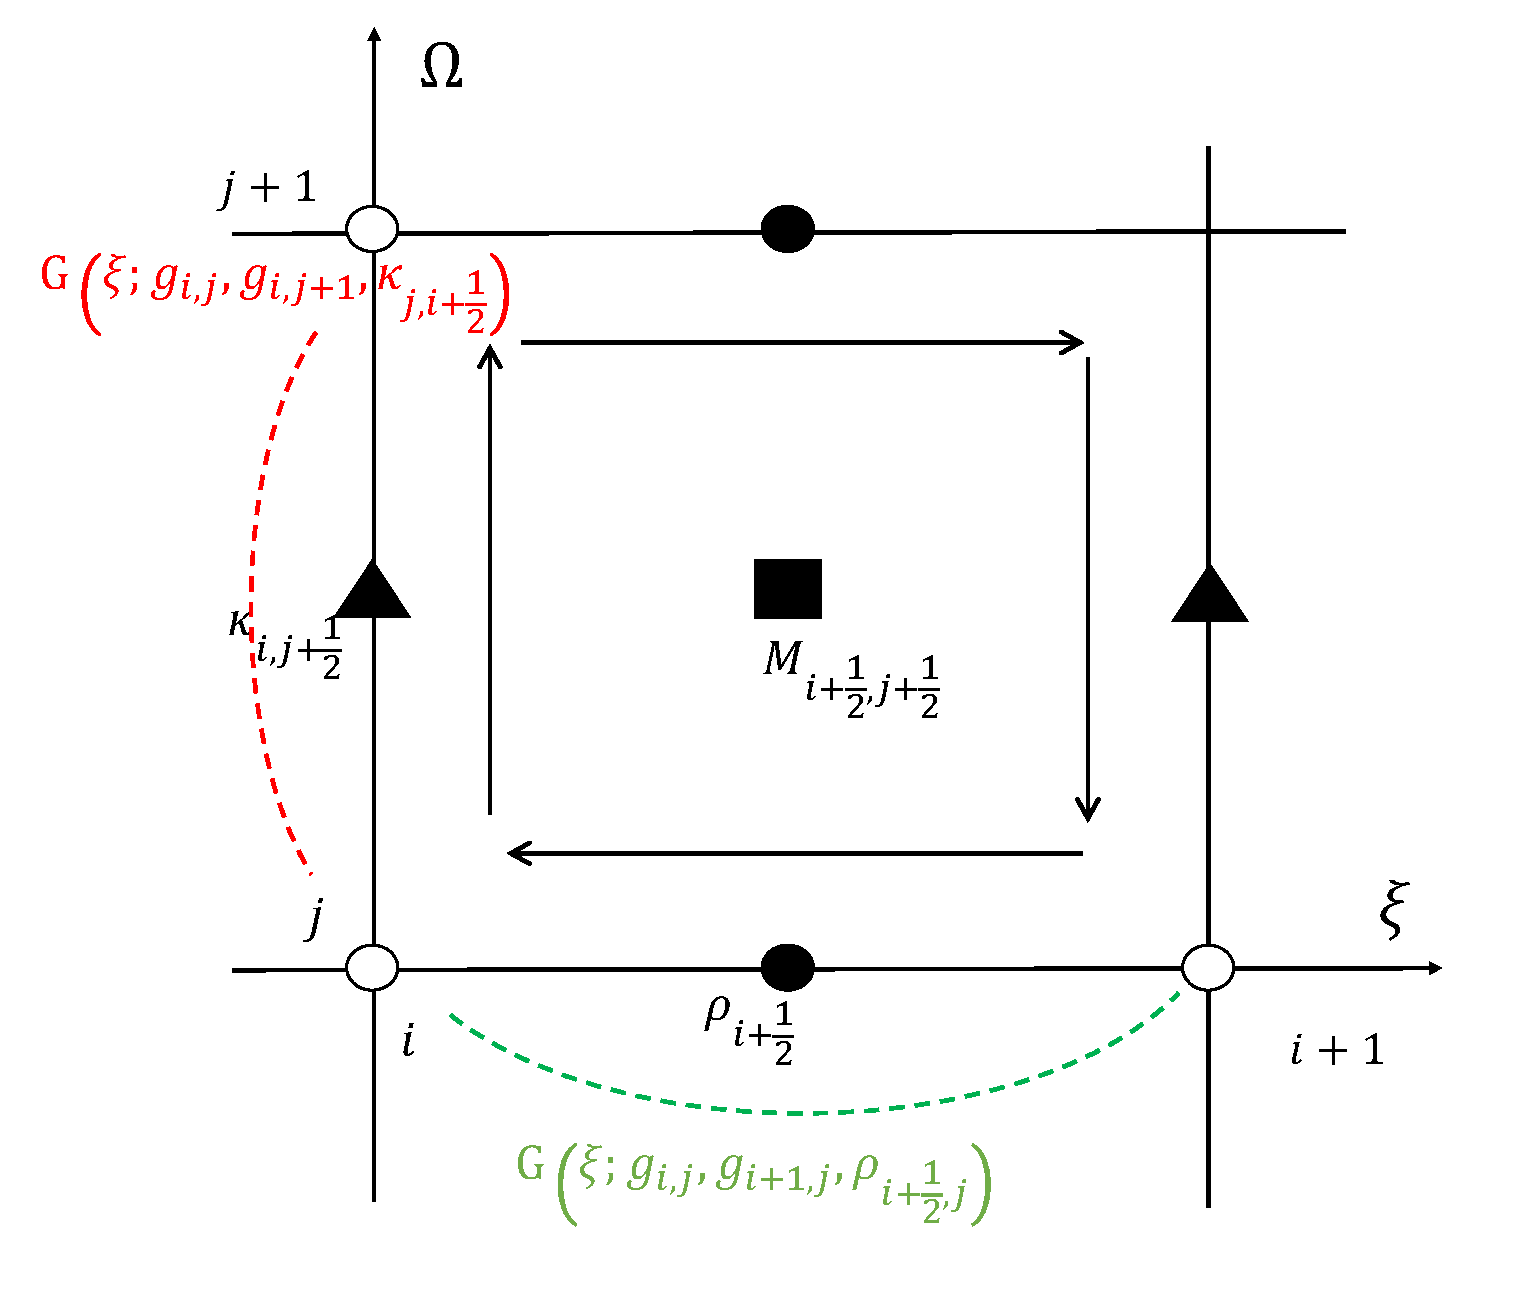
\includegraphics[scale=0.3]{cpc_img/IDO.pdf}
    \caption{The interpolating functions and  integrated values in $\xi,\Omega$ domain.}
    \label{fig.grids}
\end{figure}
%The interpolation relies on the line integrated values 
%The calculation at this step relies upon $\rho_{i+\frac{1}{2},j}$ and $\kappa_{i,j+\frac{1}{2}}$, which are the line integrated value of $\mathcal{F}$ 
%To solve the integral value $\rho$ and $\kappa$, we consider the  on given $j$ and $i$ grid respectively, and 
Integrating Eq.~(\ref{eq.Euler2}) along $\xi$ and $\Omega$ over the grid interval  yields the time evolution of the integral values \cite{imadera2009}
%, accroding to the definition in Eq.~(\ref{eq.intg}). The time evolution of the integral value is derived from the Vlasov equation,
\begin{equation}\label{eq.line}
    \begin{aligned}
    \left.\frac{\partial \rho}{\partial t}\right|_{i+\frac{1}{2},j} &= \int_{\xi_i}^{\xi_{i+1}}[ - m_j(\xi) \left.\frac{\partial g}{\partial \xi}\right|_{j}(\xi) + n_j(\xi) \left.\frac{\partial g}{\partial \Omega}\right|_{j}(\xi) + \mathcal{S}_j(\xi)]~\mathrm{d} \xi,
    \\
    \left.\frac{\partial \kappa}{\partial t}\right|_{i,j+\frac{1}{2}}
    &= \int_{\Omega_j}^{\Omega_{j+1}}[ - m_i(\Omega) \left.\frac{\partial g}{\partial \xi}\right|_{i}(\Omega) + n_i(\Omega) \left.\frac{\partial g}{\partial \Omega}\right|_{i}(\Omega) + \mathcal{S}_i(\Omega)]~\mathrm{d} \Omega.
    \end{aligned}
\end{equation}
%Then, enters step 2, solve Eq.~(\ref{eq.line})
%In the above integrals on the right-hand-side, We apply 
The third-order central interpolation scheme is applied to approximate the functions $m$ and $n$ along the $\xi$ and $\Omega$ dimension and the interpolating stencil is used to approximate the derivatives, 
\begin{equation}
    \begin{aligned}
       \left.\frac{\partial g}{\partial \xi}\right|_{j}(\xi)
        &\simeq G\left(\xi;\left.\frac{\partial g}{\partial \xi}\right|_{i,j},\left.\frac{\partial g}{\partial \xi}\right|_{i+1,j},g_{i+1,j}-g_{i,j}\right),
        \\
        \left.\frac{\partial g}{\partial \Omega}\right|_{j}(\xi)
         &\simeq G\left(\xi;\left.\frac{\partial g}{\partial \Omega}\right|_{i,j},\left.\frac{\partial g}{\partial \Omega}\right|_{i+1,j},    \left.\frac{\partial \rho}{\partial \Omega}\right|_{i+\frac{1}{2},j}\right),
         \\
         \left.\frac{\partial g}{\partial \Omega}\right|_{i}(\Omega) 
     &\simeq G\left(\Omega;\left.\frac{\partial g}{\partial \Omega}\right|_{i,j},\left.\frac{\partial g}{\partial \Omega}\right|_{i,j+1},g_{i,j+1}-g_{i,j}\right),\\
         \left.\frac{\partial g}{\partial \xi}\right|_{i}(\Omega) 
  &\simeq G\left(\Omega;\left.\frac{\partial g}{\partial \xi}\right|_{i,j},\left.\frac{\partial g}{\partial \xi}\right|_{i,j+1},\left.\frac{\partial \kappa}{\partial \xi}\right|_{i,j+\frac{1}{2}}\right),
    \end{aligned}
\end{equation}
%The interpolations bring new dependence on intergral value $\rho_{\Omega;i+\frac{1}{2},j}$ and $\kappa_{\xi;i,j+\frac{1}{2}}$. Therefore, 
%We apply additional interpolation functions to approximate 
%$\rho$ along $\Omega$ and $\kappa$ along $\xi$ to calculate its 
where 
%the derivatives
\begin{equation}
    \begin{aligned}
    \left.\frac{\partial \rho}{\partial \Omega}\right|_{i+\frac{1}{2},j}
    &\simeq \left.\frac{\partial}{\partial \Omega} G(\Omega;\rho_{i+\frac{1}{2},j},\rho_{i+\frac{1}{2},j+1}, M_{i+\frac{1}{2},j+\frac{1}{2}})\right|_{i+\frac{1}{2},j}~, \\
    \left.\frac{\partial \kappa}{\partial \xi}\right|_{i,j+\frac{1}{2}}
 &\simeq \left.\frac{\partial}{\partial \xi} G(\xi;\kappa_{i,j+\frac{1}{2}},\kappa_{i+1,j+\frac{1}{2}}, M_{i+\frac{1}{2},j+\frac{1}{2}})\right|_{i,j+\frac{1}{2}}~.
    \end{aligned}
\end{equation} 
%the interpolations rely both on 
%where the surface integral 
% and it can be readily transformed to the loop integral 
The time evolution of the surface integral $M_{i+\frac{1}{2},j+\frac{1}{2}}=\int_{\xi_i}^{\xi_{i+1}}\int_{\Omega_j}^{\Omega_{j+1}}g(t,\xi,\Omega)d\xi d\Omega$
% according to the Stokes theorem 
is given by \cite{imadera2009}
\begin{equation}\label{eq.area}
    \begin{aligned}
         \left.\frac{\partial M}{\partial t}\right|_{i+\frac{1}{2},j+\frac{1}{2}}
         &= \int_{\xi_i}^{\xi_{i+1}} n_{j+1}(\xi) g_{j+1}(\xi)~\mathrm{d}\xi - \int_{\Omega_j}^{\Omega_{j+1}} m_{i+1}(\Omega) g_{i+1} (\Omega)~\mathrm{d} \Omega \\
        & - \int_{\xi_i}^{\xi_{i+1}} n_{j}(\xi) g_{j}(\xi)~\mathrm{d}\xi + \int_{\Omega_j}^{\Omega_{j+1}} m_{i}(\Omega) g_{i} (\Omega) \mathrm{d}\Omega \\
        &+ \iint \mathcal{S}(\xi,\Omega)~\mathrm{d}\xi\mathrm{d}\Omega~,
    \end{aligned}
\end{equation}
where the integral of the source term is solved by trapezoidal integration.


Equations (\ref{eq.disV}), (\ref{eq.line}), and (\ref{eq.area})
are a set of ordinary differential equations that can be solved  by the RK method.
%-------------------------------%-------------------------------
For the boundary conditions, the values of the perturbed distribution vanish at the $\Omega$ boundaries
and
the distribution functions in  the resonant frame are assumed to be periodic in the  angle variable $\xi$,
\begin{equation}
    g\left(\xi,\Omega,t\right)=g\left(\xi+2 \pi,\Omega,t\right)~.
\end{equation}
Note that the periodic boundary conditions are valid only when the resonance does not deviate too far away from the initial resonance frame of reference with the most unstable frequency $\omega_l$ and wave number $k_l$.
\begin{figure}[htbp]
    \centering
    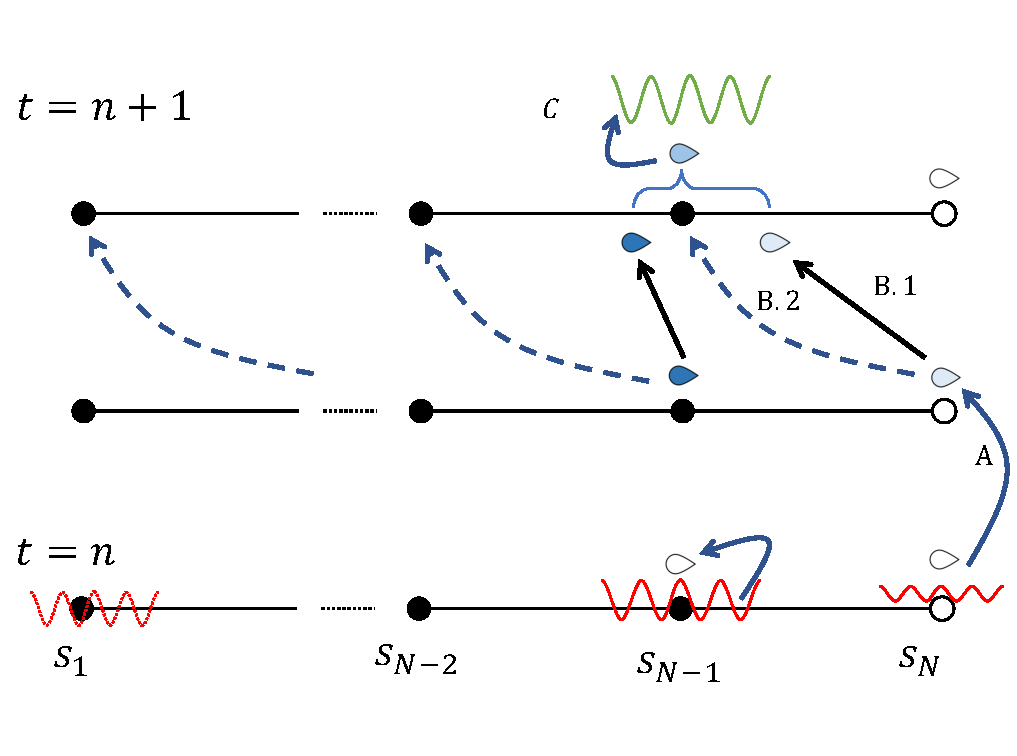
\includegraphics[scale=0.5]{cpc_img/Hybrid_demo.pdf}
    \caption{Schematic illustration of the hybrid Vlasov simulation scheme.}
    \label{fig.demo}
\end{figure}

\subsection{The Lagrangian step}
For the Lagrangian markers,
the sampling point for $\mathcal{J}$ is chosen to ensure  a uniform sampling to the initial equilibrium distribution $f_0$,
\begin{equation} 
    \mathcal{J}_l \to \int^{\mathcal{J}_l} f_0 \mathrm{d}\mathcal{J} = l/N_l~, 
\end{equation}
where $N_l$ is the total number of sampling points for $\mathcal{J}$. An illustration is shown in Fig. \ref{fig.uni_grid}(a).

To initially position the markers in the spatial domain, we place them on the fixed grid, denoted as $s_i$, which is the same grid used for solving the wave equations. To ensure that each marker updates over an identical time step, we implement nonuniform sampling, corresponding to the nonuniform wave grid. Initially, we calculate the transit time required for a marker to traverse the entire simulation domain.
\begin{equation}
    T = \int_{s_1}^{s_N} \frac{\mathrm{d}s}{v_r(s)}~
\end{equation}
where $v_r(s)$ is the local resonant velocity that has been predetermined from the background equilibrium parameter.
Then the simulation time step is set as $\Delta t = T/N$ with $N$ the total number of sampling points/grids.
Finally, the initial spatial coordinates of the markers are set according to equation (\ref{eq.resonance}) gives the trajectory of the Lagrangian marker. 
\begin{equation}
    s_{k+1} = s_k +  \int_{t}^{t+\Delta t} v_r(s_k(t)) \mathrm{d}t~
\end{equation}
where $k=1,2,3,...,N$.
The nonuniform grids with size $\Delta s$ are shown in Fig. \ref{fig.uni_grid}(b). 
Utilizing this nonuniform grid, the Lagrangian markers initially positioned on the grid advance to the next adjacent grid point after a time interval $\Delta t$.
\begin{figure}[htbp]
    \centering
    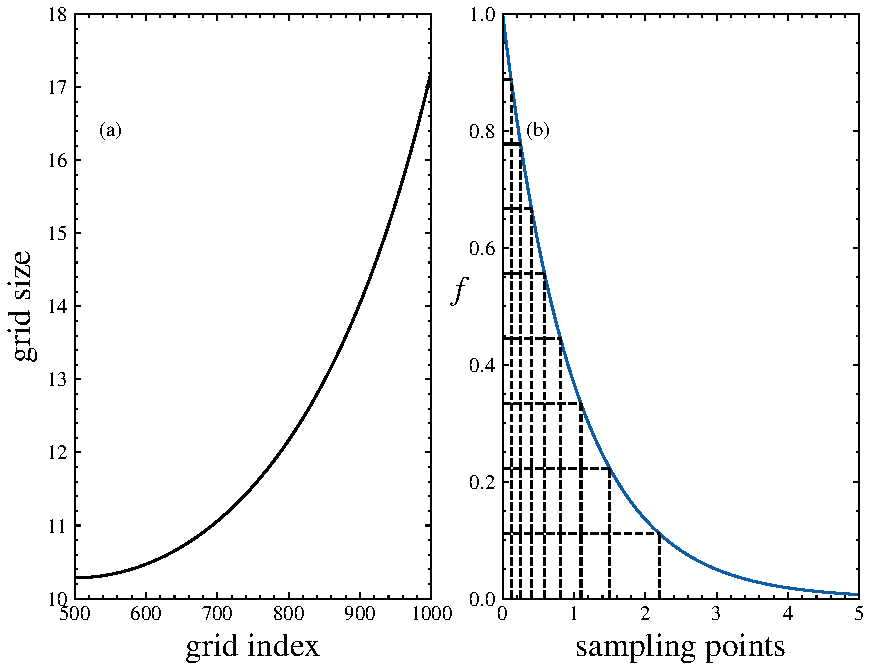
\includegraphics[scale=0.5]{cpc_img/fig_nu_grid.pdf}
    \caption{The nonuniform spatial grid obtained from resonance velocity. 
    %Here the number of grid points $N=500$.
    }
    \label{fig.uni_grid}
\end{figure}
Thus we successively push the distribution $g_{k,l}(\xi,\Omega)$  from  $s_k$ to the next grid $s_{k+1}$ for each time interval $\Delta t$.
After pushing the Lagrangian maker from the $n^\mathrm{th}$ to the $n+1^\mathrm{th}$ time step, the Hamiltonian  is re-calculated by  the  equilibrium quantities  at the new location of $s$ and $\mathcal{J}$, which are needed for evolving the distribution in $\xi-\Omega$ space at the next time step.

To mitigate the check board numerical error, we also implement a uniform grid and sample Lagrangian markers on $'s'$ to validate the effectiveness of our nonuniform grid approach.
After a given time step $\Delta t$ the markers deviated from the fixed grid, thus  we need to interpolate the distribution function and its derivatives required in the IDO scheme from the adjacent marker to the fixed $s$ grid.
These procedures closely resemble those of the semi-Lagrangian method \cite{sonnendrucker1999,cottet2018}. Following interpolation, the markers realign with the grid, and the next iteration starts from the grid point.
As shown in Fig.~\ref{fig.cmp1}, the wave amplitudes calculated from  the two approaches converge  as the smaller grid sizes are used for the uniform grid with interpolation.  
\begin{figure}[htbp]
    \centering
    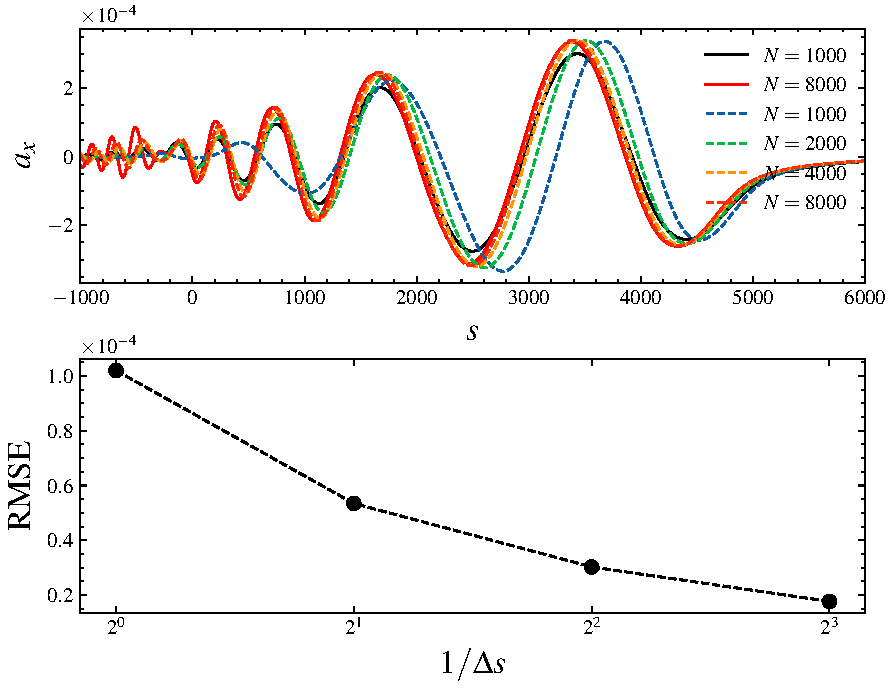
\includegraphics[scale=0.5]{cpc_img/fig_semiL.pdf}
    \caption{Wave amplitude from semi-Lagrangian method with linear interpolation of distribution at different uniform grid sizes (dashed-line) and the nonuniform grid (solid line).
    }
    \label{fig.cmp1}
\end{figure}
The evolution of $\vartheta,\mathcal{J}$ in Eq. (\ref{eq.Lagrangian}) are simply solved by applying the RK method.


Given that the evolution in the $\xi,\Omega$  phase space occurs at a significantly faster pace compared to that in the $s_i,\mathcal{J}$ domain, we employ a larger fixed time step $\Delta t$ for the Lagrangian calculations. Conversely, we employ a much smaller adaptive time step, $\Delta t_\mathrm{adp}$, for resolving the rapidly varying dynamics within the Eulerian domain. These $\Delta t_\mathrm{adp}$ are adaptively determined through real-time error analysis using the adaptive time step RK method, and satisfy
\begin{equation}
    \sum_{t=1}^T \Delta t_\mathrm{adp} = \Delta t ~.
\end{equation}
where $T$ is the total number of iterations within one $\Delta t$. 
As shown in Fig.~\ref{fig.adapetive}, 
$\Delta t_\mathrm{adp}$ is continuously adjusted and refined, consistently reducing its value whenever the numerical error exceeds the predefined error threshold. As the system undergoes nonlinear evolution, the time step $\Delta t_\mathrm{adp}$ undergoes further refinement, automatically increasing the number of iterations within a single $\Delta t$ interval. This highlights the clear advantage of adaptive hybrid methods in significantly improving computational efficiency.
\begin{figure}[htbp]
    \centering
    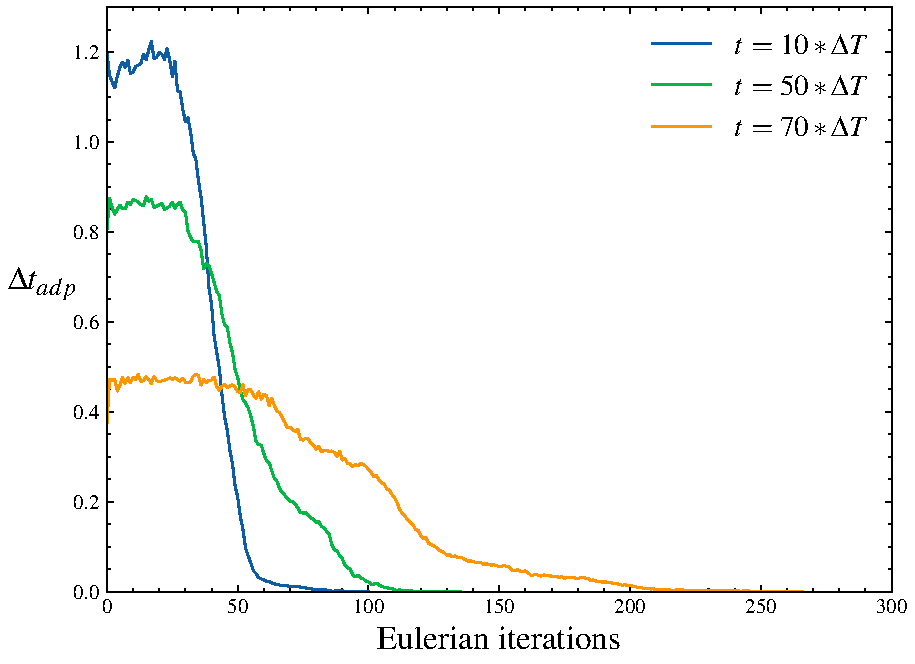
\includegraphics[scale=0.5]{cpc_img/fig_dts1.pdf}
    \caption{The variation of time step $\Delta t_\mathrm{adp}$ with the number of iterations for Eulerian calculation.  
    }
    \label{fig.adapetive}
\end{figure}


%then we sove the following envelope equation 
%explain the form
%\input{cpc/methods}
\section{Wave Equation}
\label{sec:wave}

We proceed to integrate the HEL Vlasov solver with the wave equation, enabling us to self-consistently investigate resonant wave-particle interactions. In this paper, we focus on the interaction between energetic electrons and chorus waves within the Earth's magnetosphere. Chorus waves are circularly polarized electromagnetic waves that propagate along the Earth's dipole magnetic field. The vector potential A(s, t) representing the transverse wave is expressed as follows:
\begin{equation}
    \mathbf{A}(s,t) = \mathbf{a}(s,t)e^{\imath \phi_f}~,
\end{equation}
where $\phi_f$ is the fast varying phase and $\mathbf{a}(s,t)$ is the slowly varying envelope of the wave packet. 
The second order wave equation for the chorus in the resonant frame  is 
\begin{equation}\label{eq.Wave}
    \begin{aligned}
        &\frac{\partial^2 a}{\partial t^2} - \frac{\partial^2 a}{\partial s_i^2} + {2\imath\omega_l}\frac{\partial a}{\partial t} + 2\imath k_l\frac{\partial a}{\partial s_i} + \\
        &\frac{\omega_p^2 \omega_{ce}}{(\omega_{ce}-\omega_l)} \int_0^t d \tau \frac{\partial a}{\partial \tau} e^{-\imath\left(\omega_l-\omega_{c e}\right)(t-\tau)} = {4\pi}j_p~,
        \end{aligned}
      \end{equation}
where $a = a_x + \imath a_y$ with $x$ and $y$ the directions perpendicular to the  magnetic field. 
The plasma current is a combination of contributions from both cold electrons and energetic electrons. The cold electron current can be analytically integrated. We represent the second-order wave equation (\ref{eq.Wave}) as a system of first-order ordinary differential equations, as shown below:
\begin{equation}\label{eq.Wave2}
    \begin{aligned}
        \frac{d y_0}{d t} & = y_1 + D \frac{\partial^2 y_0}{\partial s^2}
        \\
        \frac{d y_1}{d t} & =-2 \imath \omega_l y_1+\frac{\partial^2 y_0}{\partial s^2}-2 \imath k_l \frac{\partial y_0}{\partial s}- \frac{\omega^2_p\omega_{ce}}{\omega_{ce}-\omega_l}y_{2} +j_p\\
        \frac{d y_2}{d t} & =y_1-\imath\left(\omega_l-\omega_{ce}\right) y_2~,
        \end{aligned}
\end{equation}
where we have added a numerical diffusive term with $D$ the diffusive coefficient. The terms $y_0,y_1$ and $y_2$ are
\begin{equation}
    \begin{aligned}
        y_0 &= a(s_i,t)~,
        \\
        y_1 &= \frac{\partial a(s_i,t)}{\partial t}~,
        \\
        y_2 &= e^{-\imath(\omega_l-\omega_{ce})t} \int_0^t\mathrm{d}\tau \frac{\partial a}{\partial \tau} e^{\imath(\omega_l-\omega_{ce})\tau}~.
    \end{aligned}
\end{equation}

For the nonuniform, to ensure the order of precision, a linear combination of finite difference scheme is employed, and the first and second order spatial derivatives are given by 
\begin{equation}
    \frac{\partial f}{\partial z} \approx \frac{f(z_k) - f(z_{k-1})}{z_k-z_{k-1}} + \frac{f(z_k) - f(z_{k+1})}{z_k - z_{k+1}} - \frac{f(z_{k+1}) - f(z_{k-1})}{z_{k+1} - z_{k-1}}~,
\end{equation}
and
\begin{equation}
    \frac{\partial^2 f}{\partial z^2} \approx 2 \left(\frac{f(z_{k-1})}{(z_{k-1}-z_{k})(z_{k-1}-z_{k+1})}+\frac{f(z_{k})}{(z_k-z_{k+1})(z_k-z_{k-1})}+\frac{f(z_{k+1})}{(z_{k+1}-z_{k})(z_{k+1}-z_{k-1})}\right)~.
\end{equation}
The energetic electron current $j_p$ is obtained from the perpendicular velocity moment of energetic particle distribution,
\begin{equation}
    j_p(s_i,t) = - \frac{n_{h0}k_l(t)}{4\pi}\iiint \sqrt{2m_e\omega_{ce}(s)(\mathcal{J}+\Omega+\Pi_i)}f e^{\imath \xi} \rm d \xi \rm d \Omega \rm d \mathcal{J}~,
\end{equation}
where $n_{h0}$ is the density ratio of the energetic electrons to the background cold plasmas.
The coupled ordinary differential equations (\ref{eq.Wave2}) in terms of time are subsequently resolved using the RK method.

To check the contribution of the second order derivatives of slowly varying kernel $a(s_i,t)$ in the wave equation (\ref{eq.Wave}), we further simplify the integral term and obtain the first-order advective wave equation 
\begin{equation}\label{eq.Wave1st}
    \frac{\partial a}{\partial t} + v^l_{g} \frac{\partial a}{\partial s_i} = \frac{2\pi v^l_g}{k_l} j_{p}~,
\end{equation}
where $v_g^l$ is the linear group velocity.
\begin{equation}
    %a^{n+1}_k = a^{n}_k \pm {u_k} (a_{k\pm1}^{n+1} - a_{k}^{n+1})\frac{\Delta t}{\Delta s}
    \begin{aligned}
    a^{n+1}_k &= \left[ S_k^n \pm  \frac{\mathrm{imp}}{\Delta s}  {u_k} a_{k\pm1}^{n+1} + \left(\frac{1}{\Delta t} - \frac{(1- \mathrm{imp})}{\Delta s} u_k\right)  a_{k}^{n} \pm  \frac{(1-\mathrm{imp})}{\Delta s} u_k a_{k \pm 1}^{n} \right]/\left(\frac{1}{\Delta s} + \frac{\mathrm{imp}}{\Delta s}u_k\right)
    \end{aligned}
\end{equation}
where $u_k = v_g(s=s_k)$, $S_k$ is the source term in the right-hand-side of Eq. (\ref{eq.Wave1st}), $\mathrm{imp}$ is the combination factor of the implicit-explicit upwind scheme. 
The sign of the advective term depends on the direction of the group velocity. We apply absorption boundary conditions at one end of the domain and a fixed noisy initialization condition at the other end.

Fig. \ref{fig.cmp2} demonstrates that the first-order wave equation provides a strong approximation to the second-order wave equation. Consequently, the second-order term in Eq. (\ref{eq.Wave}) may be disregarded when simulating the onset of chorus wave frequency chirping for the sake of computational efficiency.
\begin{figure}[htbp]
    \centering
    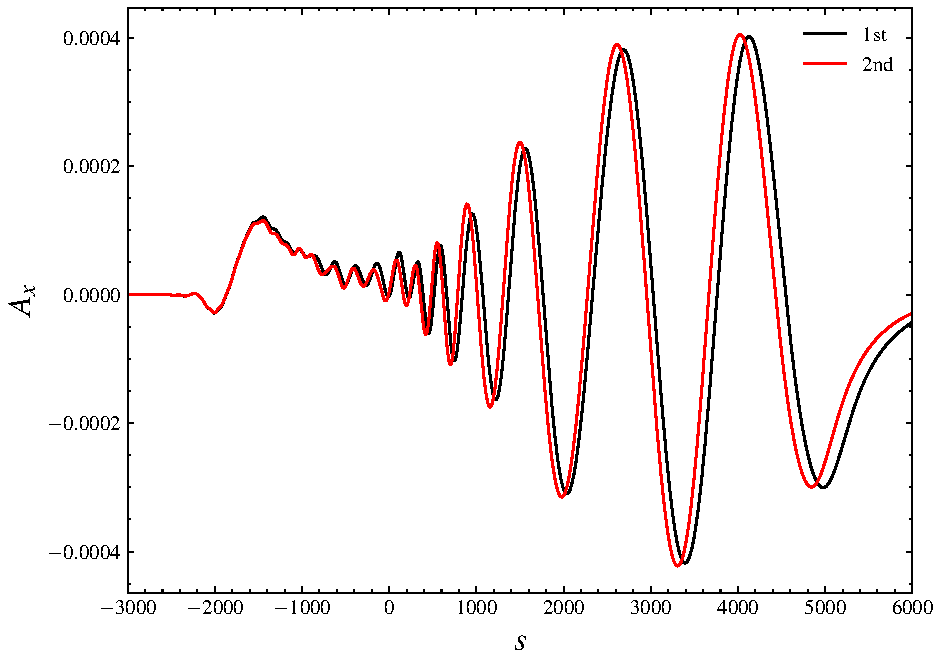
\includegraphics[scale=0.5]{cpc_img/fig_diff.pdf}
    \caption{ Wave amplitudes calculated from the second-order and first-order wave equations. 
    }
    \label{fig.cmp2}
\end{figure}

%the details of the code 
%\input{cpc/results}
\section{Benchmark Results for the Onset of Rising Tone Chorus}
\label{sec:code}
We proceed with a series of simulations, employing our method to investigate the initiation of the whistler-mode chorus. The instability of the whistler wave typically arises from the electron temperature anisotropy instability \cite{kennel1966a,kennel1966b}, and the growth rate can be derived from the linear resonance condition near $\Omega \approx 0$.

In our simulation, the energetic electron distribution is bi-Maxwellian at the magnetic equator. 
Moving away from the magnetic equator, the equilibrium distribution maintains the similar form as it does in the phase space by conventional coordinates $(s_i, p_\|, \phi, \varphi)$. The distribution function in new canonical variables is given directly by the canonical transformation in ref \cite{zheng2023a}, and we have 
\begin{equation}
    \begin{aligned}
        & f_{0}(\Omega, \mathcal{J}) =\frac{\omega_{c e 0}}{(2 \pi)^{3 / 2} v_{t h \perp 0}^2 v_{t h \| 0}} \frac{1}{1-\beta} \cdot \exp \left(-\frac{k_l^2(\Omega+\Pi_i)^2}{2 v_{t h \| 0}^2}\right) \\
        &\cdot\left(\exp \left(-\frac{(\mathcal{J}+\Omega+\Pi_i) \omega_{c e 0}}{v_{t h \perp 0}^2}\right)-\exp \left(-\frac{(\mathcal{J}+\Omega+\Pi_i) \omega_{c e 0}}{\beta v_{t h \perp 0}^2}\right)\right)~,
        \end{aligned}
\end{equation}
where $\beta$ is the depth of the loss cone, the subscript $0$ denotes the magnetic equator.

As a realistic model for the magnetosphere, the magnetic field can be approximated as a dipole field, and the major component of the background magnetic field near the equator can be approximately represented by a parabolic function \cite{tao_numerical_2014}
\begin{equation}
    B(\lambda) = B_0(1+ R_a \lambda ^2)~,
\end{equation}
where $R_a$ is the inhomogeneity ratio of the magnetic field, $B_0$ is the magnetic field strength at the equator, and $\lambda$ is the magnetic latitude. The distance alone the magnetic field line $s$ satisfies $s = L R_E \lambda$.
The background electron density is found to fit a power law form \cite{denton2004},
\begin{equation}
    n(\lambda) = n_0 (1+R_b \lambda^2)~
\end{equation}
where $R_b$ is a fitting parameter in an order of one.

\subsection{Simulation configuration}
In conventional PIC simulations, the inhomogeneity ratio $R_a$ was often enlarged by one or two order of magnitudes to reduce the simulation cost.
However, one of the advantages of our numerical scheme is that we can use realistic parameters for the Earth's dipole field.
The basic parameters of our simulation are given in Tab. (\ref{tab.parameters}).
\begin{table}\label{tab.parameters}
    \centering
    \caption{Magnetic field and plasma parameters used in the simulation.\newline}
    \begin{tabular}{lc}
    \hline
     L-shell of the magnetic field line  & 5 \\
     Magnetic field inhomogeneity ratio $R_a$ &  4.5 \\
     Background cold plasma density inhomogeneity ratio $R_b$ &  1.0 \\
     Background electron gyro frequency and plasma frequency & \makecell{ $\omega_{ce} = 0.2$\\$\omega_{pe} = 1$  }\\
     Density ratio between energetic and cold  electrons at the magnetic equator &  0.002 \\
     Parallel and perpendicular thermal velocity of energetic electrons & \makecell{$v_\perp = 0.3 c$\\ $v_\| = 0.15c$}  \\
    Depth of the loss cone $\beta$ & 0 \\
    Size of the simulation domain  & \makecell{$\lambda \in [-15^\circ, 15^\circ]$ \\ $s \in [-6115,6115] c/\omega_{pe}$} \\
    \hline
    \end{tabular}\\
    \end{table}
%(useless) Note that, since we apply the electron plasma frequency $\omega_{pe0}$ at the equator for time normalization, the value always be 1 desites the L-shell value, which gyrofrequency is dynamcally changes.
The profile of the background parameter is shown in Fig. \ref{fig.profile}.
    \begin{figure}[htbp]
        \centering
        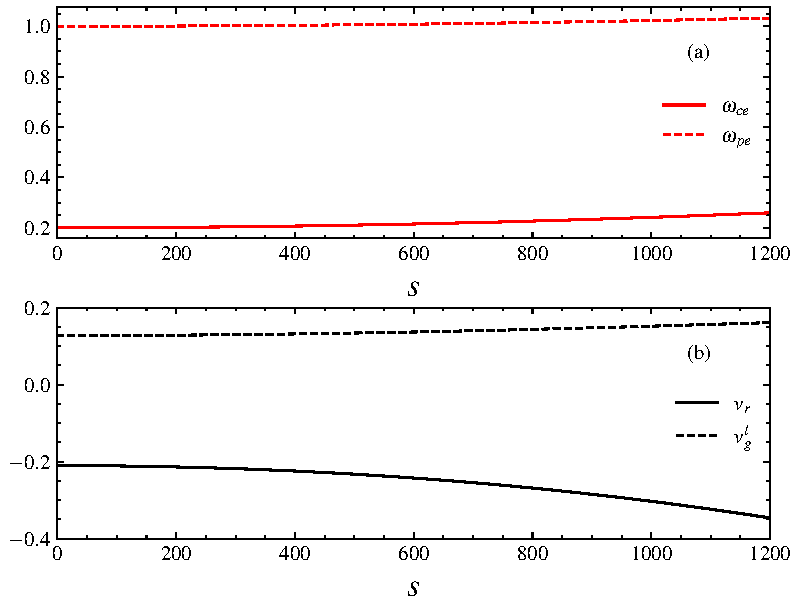
\includegraphics[scale=0.5]{cpc_img/fig_profile.pdf}
        \caption{(a) Background magnetic field and density profile. (b) Characterastic velocity in our simulation.}
        \label{fig.profile}
    \end{figure}
Meanwhile, we show the most unstable wave frequency applied in the simulation for the determination of initial reference frame. According to the choosen parameter in Tab. (\ref{tab.parameters}) and the definition of growth rate  $\gamma_l$ at the equator
\begin{equation}
\begin{aligned}
    \gamma_l(s) & =\frac{\sqrt{2 \pi} \omega_{c e} v_g \omega_{h 0}^2}{4 k_l^2 v_{t h \| 0}} e^{-\frac{\left(\omega_l-\omega_{c e}\right)^2}{2 k_l^2 v_{t h \| 0}}}
    \cdot \left((1+\beta) \frac{T_{\perp 0}}{T_{\| 0}} \frac{\omega_{c e 0}-\omega_l}{\omega_{c e 0}}-1\right)
    \end{aligned}
\end{equation}
The most unstable frequency is $\omega_l = 0.061$ and the corresponding growth rate is $\gamma_l \simeq 3.24\times 10^{-4}$, as shown by a scan of the parameter given in Fig.~\ref{fig.para}.
\begin{figure}[htbp]
    \centering
    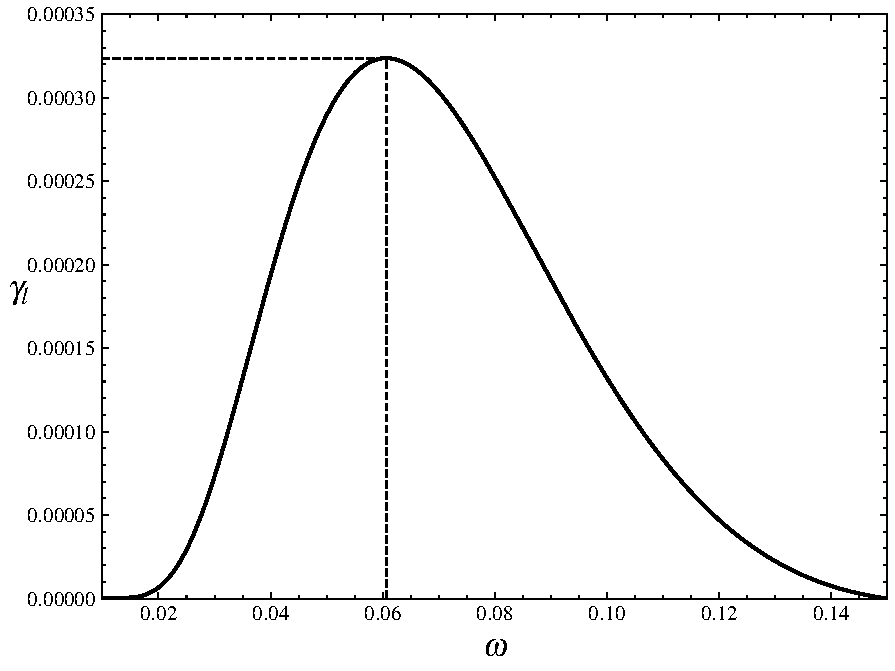
\includegraphics[scale=0.5]{cpc_img/fig_gamma1d.pdf}
    \caption{Linear growth rate $\gamma$ with respect to $\omega$ in the chosen parameter. The initial frequency of the wave is obtained from the most unstable frequency indicated by the vertical black line.}
    \label{fig.para}
\end{figure}

Benefiting from the scale-separated numerical scheme we set the number of grids for wave solver to 1001, aligning it with the number of sampling points in $s$.
In the $\mathcal{J}$ dimension, we employ a delta function, necessitating only a single sampling point for $\mathcal{J}$. In the case of a non-delta distribution, tens of sampling points prove sufficient for $\mathcal{J}$ sampling.
As to the $\xi,\Omega$ domain, the Eulerian grids are $31 \times 401$ for $\xi \in [0,2\pi]$ and $\Omega \in [-0.1,0.1]$.

The wave is resolved within a reduced-dimensional space, leading to a relatively manageable workload, as is the case with the Lagrangian solver. However, the bottleneck occurs within the Eulerian solver, primarily due to its two-dimensional space, necessitating hundreds of iterations for a single Lagrangian time step for all markers. Nonetheless, the computational cost remains reasonable in comparison to conventional PIC simulations, where the number of sampling points is at least several orders of magnitude greater than in our method. Consequently, their simulations require several billion particles \cite{nogi2022,katoh2016}, but the phase space resolution is significantly lower than ours.

\subsection{Benchmarks results}
The linear physics are quantitatively verified in Fig. \ref{fig.linear}, where we calculate the growth rate and the velocity of the maximum wave amplitude location before nonlinear effects become dominant. In the case of the propagating wave, we determine the trajectory of the wave packet using the integral of the group velocity,
\begin{equation}
    s(t) = s(0) + \int_0^{t} v_g(s(\tau)) \mathrm{d} \tau~.
\end{equation}
Here we trace the movement of the maximum amplitude point. Its propagation is in accord with the linear group velocity, as shown in Fig. \ref{fig.linear}(a). 
For the wave peak, it indeed propagates in the linear group velocity during the linear stage.
Moreover, we estimate the amplitude growth of the wave peak along its propagation path, the growth rate is given by \cite{nogi2022}
\begin{equation}\label{eq.gm_ver}
        \Gamma = \frac{1}{t_1-t_0}\log\frac{|a(s_1,t_1)|}{|a(s_0,t_0)|}~,
\end{equation}
where $s_0,t_0$, $s_1,t_1$ are along the prppagation path.
The growth of the amplitude along the propatation path is shown in Fig. \ref{fig.linear}(b). The corresponding growth rate from equation (\ref{eq.gm_ver}) is $\Gamma_0 \simeq 3.21\times10^{-4}$, agrees well with the theoretic linear growth rate shown in Fig. \ref{fig.para}.
The results show the correctness of our simulation at linear stage.
\begin{figure}[htbp]
    \centering
    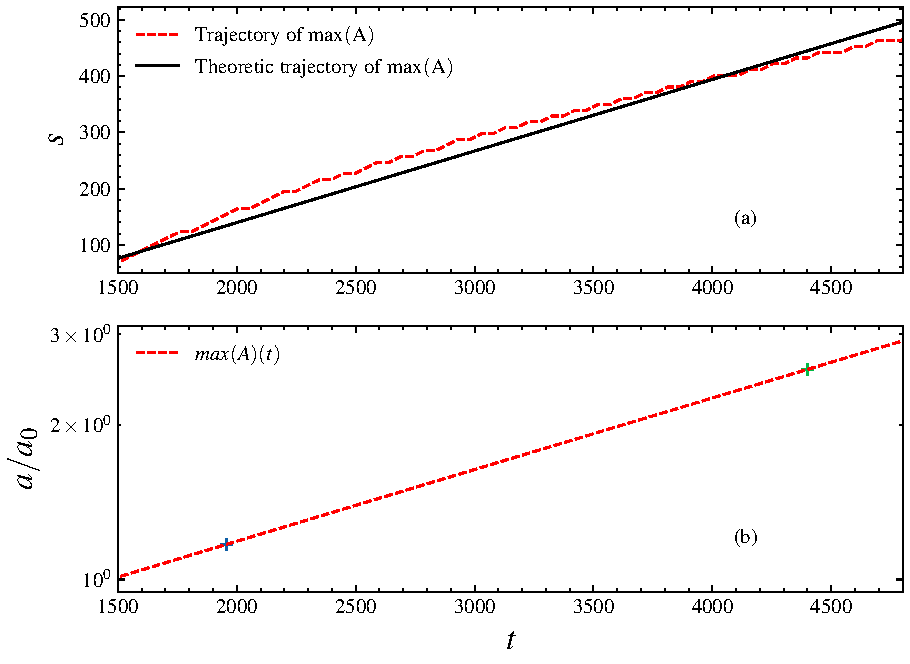
\includegraphics[scale=0.5]{cpc_img/fig_linear.pdf}
    \caption{Figure (a) is the propagation velocity of the linear wave packet with the maximum amplitude. Figure (b) denotes the growth of the wave peak amplitude with time along wave propagation path. The green cross marks the point used to caluclate the growth rate.}
    \label{fig.linear}
\end{figure}

In the nonlinear stage, the distribution of trapped electrons forms a  hole structure in $\xi-\Omega$ phase space. This phase space hole contributes to the nonlinear current, which in turn triggers the nonlinear frequency-chirping chorus wave. 
% The Hamiltonian for the resonant electrons has the form %\cite{}
% \begin{equation}
% H = \frac{k^2\Omega^2}{2} + \frac{\omega_b^2}{k^2}\left(\cos \xi + \alpha \xi \right)~,
% \end{equation}
The trapped electron experiences  an osillatory force from the wave and a noninertial force from background inhomogeneity. The forces can be described by a potential well with the form $\sin \xi + \alpha \xi$ with the parameter $\alpha$ as an inhomogeneity ratio \cite{omura2008,tao2020}.
% \begin{equation}\label{eq.alp}
%     \alpha \equiv \frac{1}{\omega_{b}^2}\left[\left(1 - 2\frac{v_r}{v_g}\right)\frac{\partial \omega}{\partial t}  -v_r^2 \frac{\partial k}{\partial s}+ \frac{\mathrm{\partial} \omega_{ce}}{\mathrm{\partial} s}\frac{k_i}{m_e}\mathcal{J}\right].
% \end{equation}
From 
the inflection point of the potential well,
%the potential well, 
we can find the X point of the phase space trajectory, 
\begin{equation}
    \xi_\mathrm{x} = - \arcsin \alpha,
\end{equation}
and the C point of the trajectory is obtained from the energy on the separatrix $e_\mathrm{spx} = \sin \xi_\mathrm{x} + \alpha \xi_\mathrm{x}$,
\begin{equation}
    \sin \xi_\mathrm{c} + \alpha \xi_\mathrm{c} = e_\mathrm{spx}.
\end{equation}
The shape of the hole, specifically its boundary, can be analytically described as follows \cite{omura2008}:
\begin{equation}\label{eq.Omega_b}
    \Omega(\xi) = \pm \frac{\omega_b}{k^2} \sqrt{2 (e_\mathrm{spx}-\cos \xi - \alpha \xi)}~,
\end{equation}
where $k$ is the wave number and $\omega_b$
%\equiv \sqrt{k^2 v_\perp a}$ 
is the trapped particle bounce frequency.
Using
the simulation data we obtain the values of $k \simeq 0.649$, $\omega_b \simeq 0.007$, and $\alpha \simeq 0.08$ at a specific location $s\simeq 2107$. Then the boundary of the hole can be obtained using Eq. (\ref{eq.Omega_b}).
As shown 
in Fig.~\ref{fig.hole},
the shape of the hole in the nonlinear simulation
closely matches  the theoretical predictions.
%we present a typical electron phase-space hole observed at a specific location $s$ in the late nonlinear stage. We determine the corresponding values of $k \simeq 0.649$, $\omega_b \simeq 0.007$, $\alpha \simeq 0.08$ based on the simulation data at that location. Additionally, we illustrated the boundary of the hole using the equation (\ref{eq.Omega_b}). Notably, the shape of the hole closely aligns with the theoretical predictions.

\begin{figure}[htbp]
    \centering
    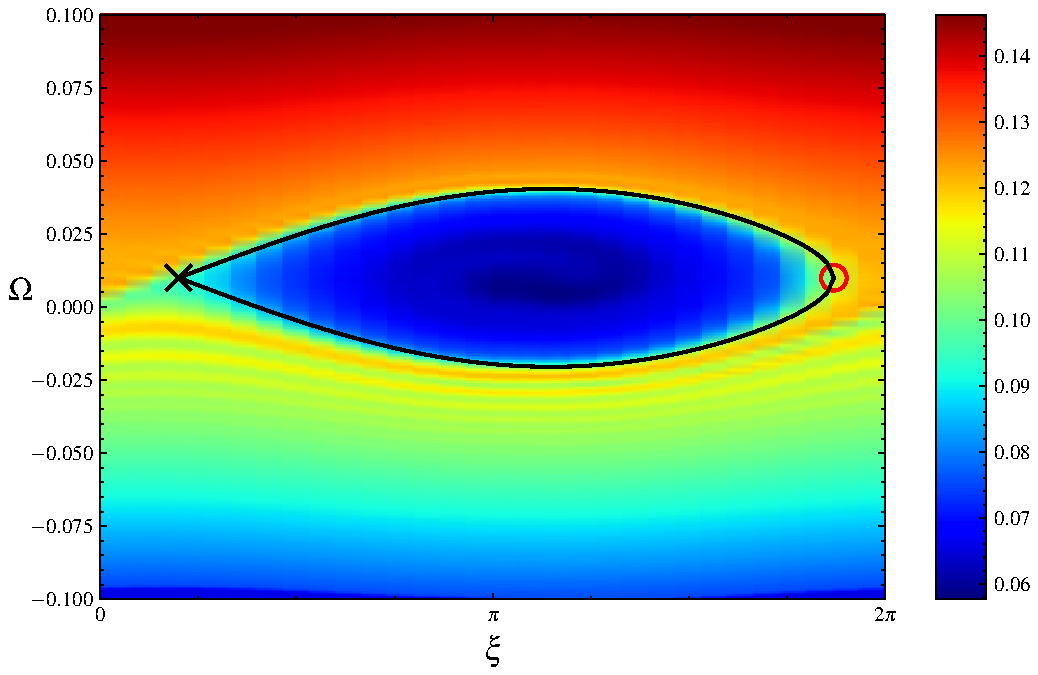
\includegraphics[scale=0.5]{cpc_img/fig_hole.pdf}
    \caption{Phase-space hole  formed by trapped electrons at $s\simeq 2107$ in the wave field. The X, C points on the left and right ends and the boundary of the hole (black solid line) are obtained from theory.}
    \label{fig.hole}
\end{figure}




\section{Conclusion}
\label{sec:end}
In summary, we have developed a hybrid Eulerian-Lagrangian method tailored for the resonance tracking Vlasov system
for the understanding of nonlinear resonant wave-particle interactions in inhomogeneous magnetic fields. This method effectively separates the perturbed wave-particle interactions within the fast varying Hamiltonian phase space while  advancing Lagrangian markers within the slowly varying Hamiltonian phase space. To validate the method, we have conducted self-consistent simulations focusing on the whistler-mode chorus in the Earth's magnetosphere  using realistic parameters. The results not only exhibit  agreement with the linear prediction  but also reveal high-resolution phase space structures of resonant energetic particles.
%The implications of this research are profound, spanning a spectrum of scientific disciplines, including fusion research, space physics, and astrophysics. This advancement in our understanding of nonlinear wave-particle interactions within inhomogeneous magnetic fields holds the potential to revolutionize our capacity to control and manipulate plasma behavior. This, in turn, can pave the way for progress in energy generation, propulsion, and space exploration. Thus, this paper represents a pivotal milestone in unlocking the untapped potential of nonlinear plasma physics within complex magnetic field environments.

%\input{cpc/appendix}

\bibliographystyle{model1-num-names}
\bibliography{nonlinear_cpc}

\end{document}

%%
